% bio.tex

\chapter{Biological Preliminaries}

\section*{Introduction}

Even if limited in scope to genome architecture, a satisfactory discussion of relationships between cell state and regulation would
be too voluminous for this document.  In the following chapter, we will attempt to cherry-pick topics and recent
developments from genetics and molecular biology to develop an intuition about chromatin architecture and the implications
of a shifting interaction map.  Readers are strongly encouraged to consult a molecular biology text, such as Molecular Biology of the Cell by
Alberts \citep{alberts2002}, for a more in depth discussion afforded here.

This chapter begins with a discussion of each actor influencing and influence by nuclear architecture.  Subsequently, the experiments
to investigate this archetype are introduced, and Hi-C is discussed in detail.  Finally, a theoretical discussion concerning
fragility in the genome presents a backdrop in which to interpret the results of our analytical experiments.

\section*{Building from the Basics}

It is difficult to overstate the importance of chromatin topology.  The morass of nucleic acids and proteins packed tightly inside the
nuclear envelope somehow contain all the information required for cell function and proliferation.  The central dogma of molecular biology,
outlined in the notes of Francis Crick `Ideas on Protein Synthesis' in 1956 \citep{crick1970} eloquently illustrates the flow of
information from primary sequence through protein.  At the highest level, the central dogma strongly reinforces the importance of
\gls{DNA} sequence content, readability, and expression.

\begin{figure}[b]
  \centering
  \caption{The original central dogma of molecular biology \citep{crick1970}}
  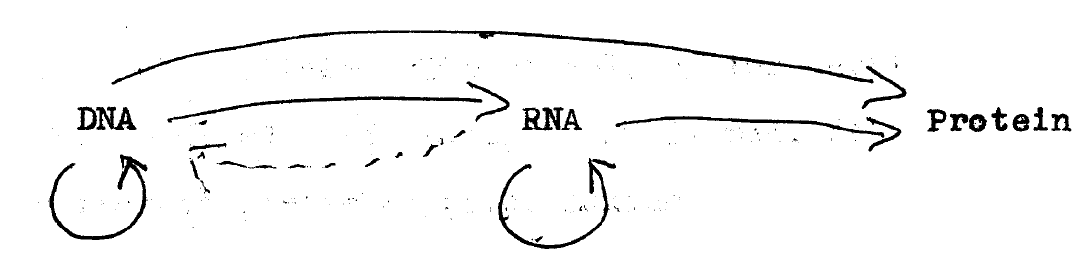
\includegraphics[width=\textwidth]{figures/biology/dogma}\label{fig:dogma}
\end{figure}

The sheer complexity of the nucleus is best decomposed into a structural hierarchy with several layers of granularity: the primary
sequence of \gls{DNA} base pairs, architectural modeling proteins, transcription factors and other binding proteins, and \glspl{CT}
and other macro molecular chromatin structures.

Ironically, the smallest nuclear resolution is the most well studied: the primary sequence of nucleic acid bases that compose the \gls{DNA}
molecule itself.  A single level of abstraction above the primary sequence considers interactions between \gls{DNA} and  architectural
proteins such as histones.  Further up the abstraction hierarchy are \gls{epigenetic} interactions, literally `above genetics',
a loose classification of secondary modifications to \gls{DNA} and architectural proteins that are characteristic of cell type and state.
Finally, chromosomes and chromosomal territories comprise the highest domain of nuclear architecture.  This conceptual hierarchy is useful
to keep in mind when investigating the origin of gene expression changes, differentiation, or disease states.

\subsection*{The Primary Sequence}

The fundamental informational unit of the cell is the \gls{nucleotide}, often called a nucleotide base or \gls{bp} when joined in a
molecule or strand.  Eukaryotic cells have a principle four character alphabet of nucleotides, distinguished by their \glspl{nucleobase}:
adenine, cytosine, guanine, and thymine.  These nucleotides are affixed to a phosphate backbone in a long, coiling polymer chain.  The
famous publication of the structure of \gls{DNA} in 1953 by researchers James Watson and Francis Crick demonstrates these polymers
exist in the nucleus as double helices \citep{watson1953}.  Hydrogen bonds between opposing nucleotides hold the double helix together in solution.
Nucleotides are classified based on the structure of the nucleotide base as purine or pyridine bases.  Adenine and guanine are purine bases,
while thymine and cytosine are pyridine bases.  \gls{DNA} bonds form between complementary nucleotides from opposite groups: adenine and thymine form
two hydrogen bonds and guanine and cytosine form three hydrogen bonds between their bases.  Thus, one half of the helix completely
determines the other half and perturbations of this structure may lead strand mutations \citep{cox2008}.

One cannot ignore the constituents of the primary sequence, particularly when considering macroscopic properties of the genome.  The nucleotide content and
order can change local sequence flexibility directly (by encoding binding sites) or indirectly (by supporting the binding of histones)
modulates the binding of important architectural proteins \citep{travers2004}.  Although a \gls{DNA} strand is a helical structure, it is an intrinsically
flexible molecule.  A naive calculation reveals that the human genome is roughly two meters in length%
\footnote{%
  A diploid human genome consists of two copies of the $\sim3.1Gb$ DNA molecule, based off estimates from the \gls{NCBI} human genome reference build 37.
  Each base pair is assumed to be roughly $0.34\times10^{-9}m$.  The entire length is $2(0.34 \times 10^{-9})(3.2 \times 10^9) = 2.176m$.
},
yet the entire genome fits into a nuclear volume of $\sim523\mu{}m$ \citep{marks2011}.  Loops as small as 100 bases in length have been
reported in enhancer and repressor element activation pathways \citep{wong2008}. These loops can form independently of proteins \citep{vafabakhsh2012}.
Altogether, \gls{DNA}'s inherent flexibility is the foundation for  many complex higher order chromatin structures.

For completeness, we note that cytosine may undergo methylation, also known as \gls{DNA} methylation or GC methylation to distinguish it
from a histone modification of the same name \citep{bird2002}.  \gls{DNA} methylation is an important epigenetic mark, involved in imprinting,
\gls{X-inactivation}, and heritable epigenetic states \citep{law2010}.  In mammals, \gls{DNA} methylation occurs almost exclusively along
symmetric \gls{GC} dinucleotides, and is estimated to occur at $\sim70-80\%$ of the \gls{GC} sites throughout the genome \citep{ehrlich1982,law2010}.
In the context of global chromatin architecture, \gls{DNA} methylation is thought to change chromatin conformation by recruiting histone
de-acetylaces \citep{schubeler2000}, suppressing large domains as in X-inactivation, recruiting architectural proteins directly \citep{yu2000},
and inhibiting transcription \citep{kass1997}.

\subsection*{Epigenetics And Chromatin Modeling}

How a \gls{DNA} molecule is packaged and condensed within a cell nucleus remains one of the basic questions of cell biology.  Intellectual curiosity aside,
why is it so important to unravel the chromosomal architecture?  Researcher J.C. Hansen notes, `In biology, structure is inexorably linked to function.' \citep{hansen2012}
The pursuit of an accurate \textit{\gls{in vivo}} model for \gls{DNA} and protein packaging continues to persist today, despite a legacy of experimental,
conceptual, and mathematical models.

In 1974, Kornberg discovered that chromatin contained roughly equal amounts of \gls{DNA} and protein \citep{kornberg1974}.  A year later, Pierre Chambon
and colleagues described the separation of chromatin into protein complexes spaced evenly on the \gls{DNA} molecule as `beads on a string.' \citep{oudet1975}
The observed beads are nucleosomes, bundles composed of a histone octamer and $\sim200$ bases (later reported to be $167$ bases) \citep{robinson2006} of
coiled \gls{DNA}. Much as the nucleotide is the fundamental unit of the genome, nucleosomes are the fundamental units of the epigenome.  Nucleosomes in
series are called a \gls{nucleosome array}.  A nucleosome consists of two components: a core particle wrapping $\sim146$ base pairs of DNA, yielding a
6 fold compaction in length, and a linker portion of varying length of $0$ to $\sim80$ base pairs.  The linker component connects adjacent nucleosomes
in a nucleosome array \citep{wu2007, hansen2012}.  These arrays are $10-nm$ in diameter, provoking them to be often called the `$10-nm$' fibers.

Despite decades of research on nucleosome arrays, their structural conformation \textit{\gls{in vivo}} remains enigmatic.   Does a higher order structure
exist beyond the $10-nm$ fiber?  Nucleosome arrays and linker histones suspended in ionic solution fold naturally into a $30-nm$ fiber \citep{tremethick2007};
however, it is unclear whether this motif forms \textit{\gls{in vivo}} and its conformation may be different in the nuclear context \citep{bian2012}.
The $30-nm$ fiber model is appealing as it readily explains the highly compacted structure of mitotic chromosomes.  To form the fiber, arrays of nucleosomes
are arranged in a solenoid or double-helix structure (for full review, see Grigoryev and Woodcock \citep{grigoryev2012}).  Whether one or both structures
are present in sub-chromosomal architectures is still an open question \citep{song2014}.  Recently, experiments using cryogenic electron microscopy
(cryo-EM) suggested an alternative fractal arrangement of $10-nm$ fibers, without invoking a higher organizational unit \citep{nishino2012,hansen2012}.
It likely that a mixture of these organizational schemas exist in the cell.  Further research as needed to assess the biological relevance of the $30-nm$ fiber in
both interphase and mitotic chromosome structure.

The nucleosome core particle is a central actor controlling gene expression through local transcription regulation.  It is well established that nucleosomes
cause an attenuation of gene expression when present at physiological concentrations \citep{brown1984, lorch1987,laybourn1991,juan1994}. How
then does the cell maintain some genes as actively transcribed while others are silenced?  Nucleosomes regulate gene expression by regulating accessibility.
Gene expression is mediated by a confluence of protein-DNA interactions: enhancers bind to enhancer elements, polymerases to the \gls{TSS}, and polymerase
recruitment proteins line the promoter region to facilitate polymerase binding and transcription activation \citep{cox2008}.  At any protein-DNA junction,
local chromatin compaction can exclude binding by physically restricting access to the primary sequence.  This tightly packed form of DNA is called
\textit{\gls{heterochromatin}}, while open and accessible sequence is called \textit{\gls{euchromatin}}.

%%TODO
A critical component of gene regulation is the ability to form long range interactions between distal elements of the genome.  Enhancer or silencer elements
situated at great distances (hundreds of kilobases) from a gene promoter will form loops in the chromatin to situate that element near the target
promoter \citep{heintzman2007}.  The commonly-held view is that there are three distinctive classes of proteins facilitating gene transcription: \glspl{GTF},
promoter-specific activators, and coactivators.  \glspl{GTF} form on the promoter region, to form a \gls{PIC}, called the \gls{core promoter}.  While the
\gls{core promoter} assembly is enough to detect a basal level of transcription, often activators, proteins bound to regulatory regions upstream, downstream,
or even in neighboring genes, are recruited to the promoter region to facilitate greater level of transcription, forming long chromatin loops \citep{ptashne1997}.
Coactivators function as intermediaries in the assembly of the promoter complexes, binding both the activators and the \gls{PIC} to achieve faster throughput of
gene expression.

\subsection*{Chromosomes are organized in territories}

The highest level of genome organization is the \gls{CT} or chromosome neighborhood \citep{cremer2001}.  The hypothesis that chromosomes are segregated into
nuclear sub-volumes dates back more than 100 years \citep{cremer1993}.  The raison d'etre for these territories is not well understood; however, it is proposed
that \gls{CT} distribution in the nucleus protects the gene-rich chromosomes by localizing them to the nuclear center \citep{boyle2001, federico2006}.
\glspl{CT} create gene expression `pockets' with localized transcriptional and repair machinery \citep{bolzer2005}, and may have cell type specific positioning.

% TODO Are the chromosomal territories inherited throughout progeny?
% http://ac.els-cdn.com/S0092867403001892/1-s2.0-S0092867403001892-main.pdf?_tid=ccd0bd28-a889-11e4-9e90-00000aab0f26&acdnat=1422627232_949e19f69451fec3a919f3039a1c2a70

To date, there is no evidence to support a deterministic ordering of chromosomes in the nucleus.  However, there may exist certain deterministic rules to
chromosomal positioning.  In all human cell types studied, the radial position of the chromosomes is correlated with gene density and chromosome
size \citep{sun2000,bolzer2005}.  In most cell types, gene-rich chromosomes are found in the central nuclear compartment, while gene-poor
chromosomes surround the nuclear periphery \citep{boyle2001,kozubek2005}.  However, in cell types with non-spherical nuclear shapes, chromosomal
arrangements may deviate from this pattern, possibly reflecting more specialized functions \citep{bolzer2005}.

There is strong evidence that chromosomal territories contain small decondensed regions serving as gene expression hot-spots.  Unlike bacterial chromosomes,
in which genes from the same pathway are grouped on the chromosome in units called \textit{operons}, eukaryotic genes are distributed seemingly randomly
throughout the genome \citep{jacob1961}.  It is well known that transcriptionally active chromatin compartmentalizes based on replication
timing \citep{ferreira1997,sadoni1999,thevenin2014}.  Moreover, recent observations reveal in order to facilitate transcription of genes in
a pathway, chromosomal territories co-localize functionally related genes with transcriptional machinery.  When considering only inter-chromosomal gene
pairs, Thevenin and colleagues observed that co-functioning genes exhibit significant local concentrations, regardless
of linear distance on the primary sequence \citep{thevenin2014}.

% TODO Topologically associated domans?
% http://www.ncbi.nlm.nih.gov/pmc/articles/PMC3874840/

% TODO
% What is this about chromosome neighboorhood location determines translocation outcome?

\section*{Experimental approaches to discern nuclear topology}

The field of molecular biology is advancing rapidly, propelled forth by a surge of automated techniques.  These so-called `\gls{high-throughput}'
methodologies enable biologists and bioinformaticians to generate massive data sets with relative ease, reliability, and efficiency.  The first
reference build of the human genome is a testament to their success \citep{hgsc2004}.  However, until recently, investigating chromosomal architecture
remained an exhaustively manual process, relying on fluorescence microscopy experiments and visual inspection by researchers.  It was not until 2003,
when Job Dekker and colleagues described a technique known as \gls{3C} that the study of nuclear architecture gained a high throughput methodology
 \citep{dekker2002}. Since then, a family of high-throughput capture techniques, most named a variation on `\gls{3C}', have been developed to interrogate
different resolutions and types of chromatin interactions (see Figure\ref{fig:captureTechniques}).

The original chromosome conformation capture technique developed by Dekker and colleagues provides an average measurement of the juxtaposition frequency
between two specific genomic loci in a cell population \citep{frase2014}.  This interaction frequency measurement is thought to be reflective of
the distance between two associated loci in genomic space.  The first extension of the \gls{3C} experiment, aptly named \gls{4C}, increased
the number of interrogated regions from two loci (one to one) to all loci interacting with a chosen target region (one to all) \citep{simonis2006}.  Most
recently, the Dekker lab extended the method further using biotinylated probes to assess contacts across the entire genome (all to all) \citep{berkum2010}.
The method, known as Hi-C, boasts the first truly global quantization of every genomic contact at a given time.

The conceptual idea behind chromosomal conformation capture is remarkably simple --- to assess nearby regions, the experimenter attempts to fuse
together molecules that are physically close, then determine the interaction partners of each segment of DNA captured in this fashion.  The
\gls{3C} procedure involves five steps.   Initially, a population of cells is cultured in an appropriate growth medium to a population size
of $\sim2.5 \times 10^7$ cells \citep{berkum2010}.  The entire population is treated with formaldehyde, a small chemical commonly used to fix both
cellular samples for microscopy experiments and large specimens for organismal analysis.  Formaldehyde is a mutagen known to form DNA-DNA and
DNA-protein cross-links \citep{merk1998}.  Importantly, the formaldehyde treatment covalently binds together proximal DNA and protein structures.
In the second step, the cells are homogenized and chromatin is digested by a restriction endonuclease, an enzyme that create double-strand
cuts at certain base pair sequences \citep{berkum2010}.  Digestion creates two populations of DNA fragments: fragments bound to protein/DNA
complexes, and an unbound population.  The unbound population is discarded by filtering.  In the third step, the bound double-strand sequences
are ligated, or joined together, in highly diluted concentrations. Dilution is critical to ensure ligation reactions occur only between DNA
strands bound to the same molecular complex. The result of the ligation process is a population of chimeric DNA sequences. The fourth step
reverses the cross-links and release the recombined sequences from their complexes.  The final step comprises quantifying the restriction
fragments by PCR using primers specific for the population under study \citep{simonis2007}.

In the derivative methods 4C, 5C, and Hi-C, the basic protocol remains unchanged; however, the capture and analysis of chimeric fragments varies
depending on the application.  \gls{4C} leverages a DNA microarray to systematically screen the entire genome in an unbiased manner for DNA loci
that contact a single locus \citep{simonis2006}.  The microarray is tiled with probes which match sequences $< 100$ base pairs away from a
restriction site.  Instead of performing the PCR step from the canonical \gls{3C} assay, restriction fragments are shortened with a
second restriction enzyme, circularized, and amplified by inverse PCR\@.  Amplified probes are detected by microarray \citep{simonis2006}.
\gls{5C} extends the \gls{3C} method by replacing the PCR amplification step with multiplexed ligation-mediated amplification.  Ligation-mediated
amplification is a technique to detect and amplify specific target sequences using primer pairs that anneal next to each other on the
same DNA strand \citep{dostie2006}. Critically, the 5C method only amplifies strands which are bound by two primers ligated across the DNA ligation
junction, allowing fine control over the amplified sequences through primer careful design.  Primers are designed such that forward and
reverse \gls{5C} primers are ligated across ligation junctions of select loci in the \gls{3C} library.  Furthermore, \gls{5C} primers also
contain universal tails for amplification, permitting all bound sequences to be simultaneously amplified.  Thus, through the appropriate choice of
primers, a selected genomic loci is `carbon-copied' and amplified, allowing high resolution analysis of a given target interaction \citep{dostie2006}.
The most recent derivation of the technique, Hi-C, allows comprehensive capture of all interacting segments in the genome using \gls{NGS} techniques.
To purify all interacting segments of the genome, the Hi-C protocol calls for the labeling of all junctions with biotin markers, effectively
marking each genomic junction. Like other derivative methods, Hi-C abolishes the PCR step of \gls{3C} and replaces it with filtration using
streptavidin beads to pull down chimeric DNA sequences.  The captured sequences can then be sequenced using next generation sequences or hybridized
to a microarray.  More targeted methods ChIA-PET and ChIP-loop incorporate immunoprecipitation to select complexes containing certain proteins.

\begin{figure}[h]
  \centering
  \caption{An overview of \gls{3C} methods.}\label{fig:captureTechniques}
  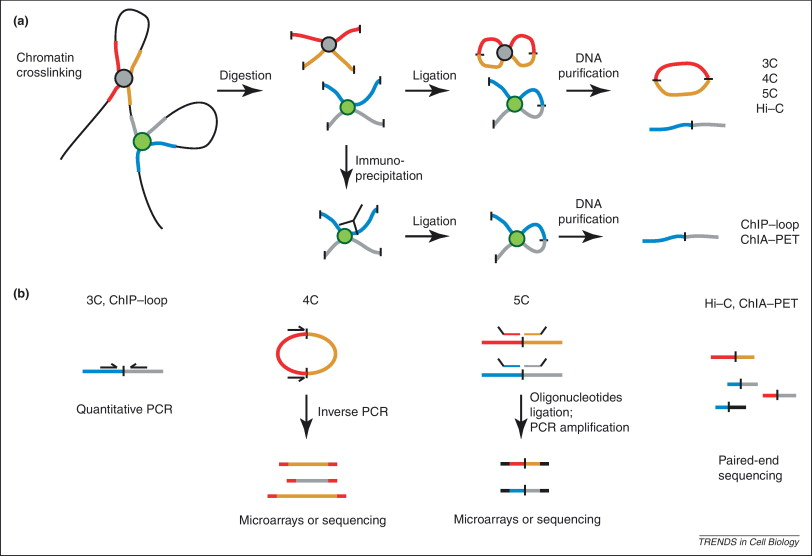
\includegraphics[width=\textwidth]{figures/biology/CompareChromosomeCapture}
  \medskip
  \small
  Here in a new line a long description about the figure, in a smaller text
  Chromatin is uniformly cross-linked and digested with a restriction enzyme.
  Bound sequences are immunoprecipitated or biotinylated, depending on the
  assay, and strands are ligated.  Ligation yields novel chimeric sequences
  which are purified.  The number of interactions are assess by qPCR in
  the canonical \gls{3C} method and ChIP-loop, inverse PCR in 4C, multiplexed
  sequencing with oligonucleotides in 5C, and paired end sequencing in Hi-C
  and ChIA-PET\@.  Adapted from Montavon et al. \citep{montavon2012}.
\end{figure}


The perceptive reader will note that much can go wrong in a \gls{3C} experiment. Every \gls{3C} method involves some level of digestion, ligation,
and amplification, and errors may be introduced at each step.  In particular, Dekker provides guidelines for three important control steps to
ensure the methodology remains integrous: control of PCR efficiency, determination of background random collisions and data
normalization \citep{dekker2006}.  Many derivative methods omit the PCR step, however all methodologies must be cognizant that
biases are introduced in any replacement protocol.

\section*{Topology and Fragility}

The first investigations into nuclear architecture were conducted by examining cell karyotypes.  Despite the development of the karyotype as a
tool for examining nuclear material in the early 20th century \citep{levitsky1924}, it wasn't until 1954 the number of chromosomes in a human
cell were definitely described \citep{tjio1956}.  Early investigations into nuclear architecture, even at the course level of a karyotype, were
hampered by technical limitations and chromosomal phenomena such as non-dysjunction and breakage.  It is not surprising that soon after the
initial description the human chromosomal number, Debakan and colleagues characterized common sites were chromosomes would undergo breakage or
translocations.  They termed these regions \gls{CFS} \citep{leyden2008}.

Many particularities render studying fragile sites difficult.  The first difficulty is semantic; chromosomal fragile sites are not precisely
defined in the literature.  When a study is performed that encompasses fragile sites, typically one of three definitions is used: regions
that are particularly sensitive to forming gaps or breaks on metaphase chromosomes \citep{glover2005}, sites where chromatin fails to compact
under mitosis \citep{leyden2008}, and non-randomly distributed loci that exhibit an increased frequency of breakage under replicational
stress \citep{franchitto2013}.  For the purposes of this discussion, a \gls{fragile site} is a region on the chromosome prone to
forming complex rearrangements, particularly double-strand breaks, repeat extensions, and translocations, when subjected to replicational stress.
These rearrangements play a pivotal role in many severely deliberating genetic diseases.

Fragile sites come in two flavors: common fragile sites (CFS) and rare fragile sites (RFS).  Fragile sites are classified into a group based on their
prevalence in the population, and the conditions under which their fragility is induced \citep{leyden2008}.  Common fragile sites are thought to be common
most chromosomes and to all humans, while rare fragile sites may be expressed in small fraction (less than 5\%) of the population \citep{wells2006}.

Rearrangements play pivotal roles in severely debilitating genetic diseases such as Fragile X Syndrome.  All males and an estimated that 60\% of females
with repeat anomalies near the FRM1 gene on the X chromosome suffer from severe mental handicap due to these alterations \citep{sutherland1995}. Additionally,
fragile sites are often found rearranged in human cancers \citep{glover2005}.  Despite these findings, the basis of fragility in fragile sites is still an
unanswered question.
